\documentclass{standalone}
\usepackage{tikz}
\usetikzlibrary{shapes.geometric}
\begin{document}
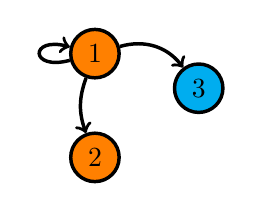
\begin{tikzpicture}
[every node/.style={inner sep=0pt}]
\node (1) [circle, minimum size=17.5pt, fill=orange, line width=1.25pt, draw=black] at (37.5pt, -25.0pt) {\textcolor{black}{1}};
\node (2) [circle, minimum size=17.5pt, fill=orange, line width=1.25pt, draw=black] at (37.5pt, -62.5pt) {\textcolor{black}{2}};
\node (3) [circle, minimum size=17.5pt, fill=cyan, line width=1.25pt, draw=black] at (75.0pt, -37.5pt) {\textcolor{black}{3}};
\draw [line width=1.25, ->, color=black, loop left] (1) to (1);
\draw [line width=1.25, ->, color=black] (1) to  [in=110, out=250] (2);
\draw [line width=1.25, ->, color=black] (1) to  [in=127, out=16] (3);
\end{tikzpicture}

\end{document}
